
% Default to the notebook output style

    


% Inherit from the specified cell style.




    
\documentclass[11pt]{article}

    
    
    \usepackage[T1]{fontenc}
    % Nicer default font (+ math font) than Computer Modern for most use cases
    \usepackage{mathpazo}

    % Basic figure setup, for now with no caption control since it's done
    % automatically by Pandoc (which extracts ![](path) syntax from Markdown).
    \usepackage{graphicx}
    % We will generate all images so they have a width \maxwidth. This means
    % that they will get their normal width if they fit onto the page, but
    % are scaled down if they would overflow the margins.
    \makeatletter
    \def\maxwidth{\ifdim\Gin@nat@width>\linewidth\linewidth
    \else\Gin@nat@width\fi}
    \makeatother
    \let\Oldincludegraphics\includegraphics
    % Set max figure width to be 80% of text width, for now hardcoded.
    \renewcommand{\includegraphics}[1]{\Oldincludegraphics[width=.95\maxwidth]{#1}}
    % Ensure that by default, figures have no caption (until we provide a
    % proper Figure object with a Caption API and a way to capture that
    % in the conversion process - todo).
    \usepackage{caption}
    \DeclareCaptionLabelFormat{nolabel}{}
    \captionsetup{labelformat=nolabel}

    \usepackage{adjustbox} % Used to constrain images to a maximum size 
    \usepackage{xcolor} % Allow colors to be defined
    \usepackage{enumerate} % Needed for markdown enumerations to work
    \usepackage{geometry} % Used to adjust the document margins
    \usepackage{amsmath} % Equations
    \usepackage{amssymb} % Equations
    \usepackage{textcomp} % defines textquotesingle
    % Hack from http://tex.stackexchange.com/a/47451/13684:
    \AtBeginDocument{%
        \def\PYZsq{\textquotesingle}% Upright quotes in Pygmentized code
    }
    \usepackage{upquote} % Upright quotes for verbatim code
    \usepackage{eurosym} % defines \euro
    \usepackage[mathletters]{ucs} % Extended unicode (utf-8) support
    \usepackage[utf8x]{inputenc} % Allow utf-8 characters in the tex document
    \usepackage{fancyvrb} % verbatim replacement that allows latex
    \usepackage{grffile} % extends the file name processing of package graphics 
                         % to support a larger range 
    % The hyperref package gives us a pdf with properly built
    % internal navigation ('pdf bookmarks' for the table of contents,
    % internal cross-reference links, web links for URLs, etc.)
    \usepackage{hyperref}
    \usepackage{longtable} % longtable support required by pandoc >1.10
    \usepackage{booktabs}  % table support for pandoc > 1.12.2
    \usepackage[inline]{enumitem} % IRkernel/repr support (it uses the enumerate* environment)
    \usepackage[normalem]{ulem} % ulem is needed to support strikethroughs (\sout)
                                % normalem makes italics be italics, not underlines
    \usepackage{mathrsfs}
    \usepackage{graphicx}
	
    
    
    % Colors for the hyperref package
    \definecolor{urlcolor}{rgb}{0,.145,.698}
    \definecolor{linkcolor}{rgb}{.71,0.21,0.01}
    \definecolor{citecolor}{rgb}{.12,.54,.11}

    % ANSI colors
    \definecolor{ansi-black}{HTML}{3E424D}
    \definecolor{ansi-black-intense}{HTML}{282C36}
    \definecolor{ansi-red}{HTML}{E75C58}
    \definecolor{ansi-red-intense}{HTML}{B22B31}
    \definecolor{ansi-green}{HTML}{00A250}
    \definecolor{ansi-green-intense}{HTML}{007427}
    \definecolor{ansi-yellow}{HTML}{DDB62B}
    \definecolor{ansi-yellow-intense}{HTML}{B27D12}
    \definecolor{ansi-blue}{HTML}{208FFB}
    \definecolor{ansi-blue-intense}{HTML}{0065CA}
    \definecolor{ansi-magenta}{HTML}{D160C4}
    \definecolor{ansi-magenta-intense}{HTML}{A03196}
    \definecolor{ansi-cyan}{HTML}{60C6C8}
    \definecolor{ansi-cyan-intense}{HTML}{258F8F}
    \definecolor{ansi-white}{HTML}{C5C1B4}
    \definecolor{ansi-white-intense}{HTML}{A1A6B2}
    \definecolor{ansi-default-inverse-fg}{HTML}{FFFFFF}
    \definecolor{ansi-default-inverse-bg}{HTML}{000000}

    % commands and environments needed by pandoc snippets
    % extracted from the output of `pandoc -s`
    \providecommand{\tightlist}{%
      \setlength{\itemsep}{0pt}\setlength{\parskip}{0pt}}
    \DefineVerbatimEnvironment{Highlighting}{Verbatim}{commandchars=\\\{\}}
    % Add ',fontsize=\small' for more characters per line
    \newenvironment{Shaded}{}{}
    \newcommand{\KeywordTok}[1]{\textcolor[rgb]{0.00,0.44,0.13}{\textbf{{#1}}}}
    \newcommand{\DataTypeTok}[1]{\textcolor[rgb]{0.56,0.13,0.00}{{#1}}}
    \newcommand{\DecValTok}[1]{\textcolor[rgb]{0.25,0.63,0.44}{{#1}}}
    \newcommand{\BaseNTok}[1]{\textcolor[rgb]{0.25,0.63,0.44}{{#1}}}
    \newcommand{\FloatTok}[1]{\textcolor[rgb]{0.25,0.63,0.44}{{#1}}}
    \newcommand{\CharTok}[1]{\textcolor[rgb]{0.25,0.44,0.63}{{#1}}}
    \newcommand{\StringTok}[1]{\textcolor[rgb]{0.25,0.44,0.63}{{#1}}}
    \newcommand{\CommentTok}[1]{\textcolor[rgb]{0.38,0.63,0.69}{\textit{{#1}}}}
    \newcommand{\OtherTok}[1]{\textcolor[rgb]{0.00,0.44,0.13}{{#1}}}
    \newcommand{\AlertTok}[1]{\textcolor[rgb]{1.00,0.00,0.00}{\textbf{{#1}}}}
    \newcommand{\FunctionTok}[1]{\textcolor[rgb]{0.02,0.16,0.49}{{#1}}}
    \newcommand{\RegionMarkerTok}[1]{{#1}}
    \newcommand{\ErrorTok}[1]{\textcolor[rgb]{1.00,0.00,0.00}{\textbf{{#1}}}}
    \newcommand{\NormalTok}[1]{{#1}}
    
    % Additional commands for more recent versions of Pandoc
    \newcommand{\ConstantTok}[1]{\textcolor[rgb]{0.53,0.00,0.00}{{#1}}}
    \newcommand{\SpecialCharTok}[1]{\textcolor[rgb]{0.25,0.44,0.63}{{#1}}}
    \newcommand{\VerbatimStringTok}[1]{\textcolor[rgb]{0.25,0.44,0.63}{{#1}}}
    \newcommand{\SpecialStringTok}[1]{\textcolor[rgb]{0.73,0.40,0.53}{{#1}}}
    \newcommand{\ImportTok}[1]{{#1}}
    \newcommand{\DocumentationTok}[1]{\textcolor[rgb]{0.73,0.13,0.13}{\textit{{#1}}}}
    \newcommand{\AnnotationTok}[1]{\textcolor[rgb]{0.38,0.63,0.69}{\textbf{\textit{{#1}}}}}
    \newcommand{\CommentVarTok}[1]{\textcolor[rgb]{0.38,0.63,0.69}{\textbf{\textit{{#1}}}}}
    \newcommand{\VariableTok}[1]{\textcolor[rgb]{0.10,0.09,0.49}{{#1}}}
    \newcommand{\ControlFlowTok}[1]{\textcolor[rgb]{0.00,0.44,0.13}{\textbf{{#1}}}}
    \newcommand{\OperatorTok}[1]{\textcolor[rgb]{0.40,0.40,0.40}{{#1}}}
    \newcommand{\BuiltInTok}[1]{{#1}}
    \newcommand{\ExtensionTok}[1]{{#1}}
    \newcommand{\PreprocessorTok}[1]{\textcolor[rgb]{0.74,0.48,0.00}{{#1}}}
    \newcommand{\AttributeTok}[1]{\textcolor[rgb]{0.49,0.56,0.16}{{#1}}}
    \newcommand{\InformationTok}[1]{\textcolor[rgb]{0.38,0.63,0.69}{\textbf{\textit{{#1}}}}}
    \newcommand{\WarningTok}[1]{\textcolor[rgb]{0.38,0.63,0.69}{\textbf{\textit{{#1}}}}}
    
    
    % Define a nice break command that doesn't care if a line doesn't already
    % exist.
    \def\br{\hspace*{\fill} \\* }
    % Math Jax compatibility definitions
    \def\gt{>}
    \def\lt{<}
    \let\Oldtex\TeX
    \let\Oldlatex\LaTeX
    \renewcommand{\TeX}{\textrm{\Oldtex}}
    \renewcommand{\LaTeX}{\textrm{\Oldlatex}}
    % Document parameters
    % Document title
    \title{Battle of Neighborhoods}
    
    
    
    
    

    % Pygments definitions
    
\makeatletter
\def\PY@reset{\let\PY@it=\relax \let\PY@bf=\relax%
    \let\PY@ul=\relax \let\PY@tc=\relax%
    \let\PY@bc=\relax \let\PY@ff=\relax}
\def\PY@tok#1{\csname PY@tok@#1\endcsname}
\def\PY@toks#1+{\ifx\relax#1\empty\else%
    \PY@tok{#1}\expandafter\PY@toks\fi}
\def\PY@do#1{\PY@bc{\PY@tc{\PY@ul{%
    \PY@it{\PY@bf{\PY@ff{#1}}}}}}}
\def\PY#1#2{\PY@reset\PY@toks#1+\relax+\PY@do{#2}}

\expandafter\def\csname PY@tok@w\endcsname{\def\PY@tc##1{\textcolor[rgb]{0.73,0.73,0.73}{##1}}}
\expandafter\def\csname PY@tok@c\endcsname{\let\PY@it=\textit\def\PY@tc##1{\textcolor[rgb]{0.25,0.50,0.50}{##1}}}
\expandafter\def\csname PY@tok@cp\endcsname{\def\PY@tc##1{\textcolor[rgb]{0.74,0.48,0.00}{##1}}}
\expandafter\def\csname PY@tok@k\endcsname{\let\PY@bf=\textbf\def\PY@tc##1{\textcolor[rgb]{0.00,0.50,0.00}{##1}}}
\expandafter\def\csname PY@tok@kp\endcsname{\def\PY@tc##1{\textcolor[rgb]{0.00,0.50,0.00}{##1}}}
\expandafter\def\csname PY@tok@kt\endcsname{\def\PY@tc##1{\textcolor[rgb]{0.69,0.00,0.25}{##1}}}
\expandafter\def\csname PY@tok@o\endcsname{\def\PY@tc##1{\textcolor[rgb]{0.40,0.40,0.40}{##1}}}
\expandafter\def\csname PY@tok@ow\endcsname{\let\PY@bf=\textbf\def\PY@tc##1{\textcolor[rgb]{0.67,0.13,1.00}{##1}}}
\expandafter\def\csname PY@tok@nb\endcsname{\def\PY@tc##1{\textcolor[rgb]{0.00,0.50,0.00}{##1}}}
\expandafter\def\csname PY@tok@nf\endcsname{\def\PY@tc##1{\textcolor[rgb]{0.00,0.00,1.00}{##1}}}
\expandafter\def\csname PY@tok@nc\endcsname{\let\PY@bf=\textbf\def\PY@tc##1{\textcolor[rgb]{0.00,0.00,1.00}{##1}}}
\expandafter\def\csname PY@tok@nn\endcsname{\let\PY@bf=\textbf\def\PY@tc##1{\textcolor[rgb]{0.00,0.00,1.00}{##1}}}
\expandafter\def\csname PY@tok@ne\endcsname{\let\PY@bf=\textbf\def\PY@tc##1{\textcolor[rgb]{0.82,0.25,0.23}{##1}}}
\expandafter\def\csname PY@tok@nv\endcsname{\def\PY@tc##1{\textcolor[rgb]{0.10,0.09,0.49}{##1}}}
\expandafter\def\csname PY@tok@no\endcsname{\def\PY@tc##1{\textcolor[rgb]{0.53,0.00,0.00}{##1}}}
\expandafter\def\csname PY@tok@nl\endcsname{\def\PY@tc##1{\textcolor[rgb]{0.63,0.63,0.00}{##1}}}
\expandafter\def\csname PY@tok@ni\endcsname{\let\PY@bf=\textbf\def\PY@tc##1{\textcolor[rgb]{0.60,0.60,0.60}{##1}}}
\expandafter\def\csname PY@tok@na\endcsname{\def\PY@tc##1{\textcolor[rgb]{0.49,0.56,0.16}{##1}}}
\expandafter\def\csname PY@tok@nt\endcsname{\let\PY@bf=\textbf\def\PY@tc##1{\textcolor[rgb]{0.00,0.50,0.00}{##1}}}
\expandafter\def\csname PY@tok@nd\endcsname{\def\PY@tc##1{\textcolor[rgb]{0.67,0.13,1.00}{##1}}}
\expandafter\def\csname PY@tok@s\endcsname{\def\PY@tc##1{\textcolor[rgb]{0.73,0.13,0.13}{##1}}}
\expandafter\def\csname PY@tok@sd\endcsname{\let\PY@it=\textit\def\PY@tc##1{\textcolor[rgb]{0.73,0.13,0.13}{##1}}}
\expandafter\def\csname PY@tok@si\endcsname{\let\PY@bf=\textbf\def\PY@tc##1{\textcolor[rgb]{0.73,0.40,0.53}{##1}}}
\expandafter\def\csname PY@tok@se\endcsname{\let\PY@bf=\textbf\def\PY@tc##1{\textcolor[rgb]{0.73,0.40,0.13}{##1}}}
\expandafter\def\csname PY@tok@sr\endcsname{\def\PY@tc##1{\textcolor[rgb]{0.73,0.40,0.53}{##1}}}
\expandafter\def\csname PY@tok@ss\endcsname{\def\PY@tc##1{\textcolor[rgb]{0.10,0.09,0.49}{##1}}}
\expandafter\def\csname PY@tok@sx\endcsname{\def\PY@tc##1{\textcolor[rgb]{0.00,0.50,0.00}{##1}}}
\expandafter\def\csname PY@tok@m\endcsname{\def\PY@tc##1{\textcolor[rgb]{0.40,0.40,0.40}{##1}}}
\expandafter\def\csname PY@tok@gh\endcsname{\let\PY@bf=\textbf\def\PY@tc##1{\textcolor[rgb]{0.00,0.00,0.50}{##1}}}
\expandafter\def\csname PY@tok@gu\endcsname{\let\PY@bf=\textbf\def\PY@tc##1{\textcolor[rgb]{0.50,0.00,0.50}{##1}}}
\expandafter\def\csname PY@tok@gd\endcsname{\def\PY@tc##1{\textcolor[rgb]{0.63,0.00,0.00}{##1}}}
\expandafter\def\csname PY@tok@gi\endcsname{\def\PY@tc##1{\textcolor[rgb]{0.00,0.63,0.00}{##1}}}
\expandafter\def\csname PY@tok@gr\endcsname{\def\PY@tc##1{\textcolor[rgb]{1.00,0.00,0.00}{##1}}}
\expandafter\def\csname PY@tok@ge\endcsname{\let\PY@it=\textit}
\expandafter\def\csname PY@tok@gs\endcsname{\let\PY@bf=\textbf}
\expandafter\def\csname PY@tok@gp\endcsname{\let\PY@bf=\textbf\def\PY@tc##1{\textcolor[rgb]{0.00,0.00,0.50}{##1}}}
\expandafter\def\csname PY@tok@go\endcsname{\def\PY@tc##1{\textcolor[rgb]{0.53,0.53,0.53}{##1}}}
\expandafter\def\csname PY@tok@gt\endcsname{\def\PY@tc##1{\textcolor[rgb]{0.00,0.27,0.87}{##1}}}
\expandafter\def\csname PY@tok@err\endcsname{\def\PY@bc##1{\setlength{\fboxsep}{0pt}\fcolorbox[rgb]{1.00,0.00,0.00}{1,1,1}{\strut ##1}}}
\expandafter\def\csname PY@tok@kc\endcsname{\let\PY@bf=\textbf\def\PY@tc##1{\textcolor[rgb]{0.00,0.50,0.00}{##1}}}
\expandafter\def\csname PY@tok@kd\endcsname{\let\PY@bf=\textbf\def\PY@tc##1{\textcolor[rgb]{0.00,0.50,0.00}{##1}}}
\expandafter\def\csname PY@tok@kn\endcsname{\let\PY@bf=\textbf\def\PY@tc##1{\textcolor[rgb]{0.00,0.50,0.00}{##1}}}
\expandafter\def\csname PY@tok@kr\endcsname{\let\PY@bf=\textbf\def\PY@tc##1{\textcolor[rgb]{0.00,0.50,0.00}{##1}}}
\expandafter\def\csname PY@tok@bp\endcsname{\def\PY@tc##1{\textcolor[rgb]{0.00,0.50,0.00}{##1}}}
\expandafter\def\csname PY@tok@fm\endcsname{\def\PY@tc##1{\textcolor[rgb]{0.00,0.00,1.00}{##1}}}
\expandafter\def\csname PY@tok@vc\endcsname{\def\PY@tc##1{\textcolor[rgb]{0.10,0.09,0.49}{##1}}}
\expandafter\def\csname PY@tok@vg\endcsname{\def\PY@tc##1{\textcolor[rgb]{0.10,0.09,0.49}{##1}}}
\expandafter\def\csname PY@tok@vi\endcsname{\def\PY@tc##1{\textcolor[rgb]{0.10,0.09,0.49}{##1}}}
\expandafter\def\csname PY@tok@vm\endcsname{\def\PY@tc##1{\textcolor[rgb]{0.10,0.09,0.49}{##1}}}
\expandafter\def\csname PY@tok@sa\endcsname{\def\PY@tc##1{\textcolor[rgb]{0.73,0.13,0.13}{##1}}}
\expandafter\def\csname PY@tok@sb\endcsname{\def\PY@tc##1{\textcolor[rgb]{0.73,0.13,0.13}{##1}}}
\expandafter\def\csname PY@tok@sc\endcsname{\def\PY@tc##1{\textcolor[rgb]{0.73,0.13,0.13}{##1}}}
\expandafter\def\csname PY@tok@dl\endcsname{\def\PY@tc##1{\textcolor[rgb]{0.73,0.13,0.13}{##1}}}
\expandafter\def\csname PY@tok@s2\endcsname{\def\PY@tc##1{\textcolor[rgb]{0.73,0.13,0.13}{##1}}}
\expandafter\def\csname PY@tok@sh\endcsname{\def\PY@tc##1{\textcolor[rgb]{0.73,0.13,0.13}{##1}}}
\expandafter\def\csname PY@tok@s1\endcsname{\def\PY@tc##1{\textcolor[rgb]{0.73,0.13,0.13}{##1}}}
\expandafter\def\csname PY@tok@mb\endcsname{\def\PY@tc##1{\textcolor[rgb]{0.40,0.40,0.40}{##1}}}
\expandafter\def\csname PY@tok@mf\endcsname{\def\PY@tc##1{\textcolor[rgb]{0.40,0.40,0.40}{##1}}}
\expandafter\def\csname PY@tok@mh\endcsname{\def\PY@tc##1{\textcolor[rgb]{0.40,0.40,0.40}{##1}}}
\expandafter\def\csname PY@tok@mi\endcsname{\def\PY@tc##1{\textcolor[rgb]{0.40,0.40,0.40}{##1}}}
\expandafter\def\csname PY@tok@il\endcsname{\def\PY@tc##1{\textcolor[rgb]{0.40,0.40,0.40}{##1}}}
\expandafter\def\csname PY@tok@mo\endcsname{\def\PY@tc##1{\textcolor[rgb]{0.40,0.40,0.40}{##1}}}
\expandafter\def\csname PY@tok@ch\endcsname{\let\PY@it=\textit\def\PY@tc##1{\textcolor[rgb]{0.25,0.50,0.50}{##1}}}
\expandafter\def\csname PY@tok@cm\endcsname{\let\PY@it=\textit\def\PY@tc##1{\textcolor[rgb]{0.25,0.50,0.50}{##1}}}
\expandafter\def\csname PY@tok@cpf\endcsname{\let\PY@it=\textit\def\PY@tc##1{\textcolor[rgb]{0.25,0.50,0.50}{##1}}}
\expandafter\def\csname PY@tok@c1\endcsname{\let\PY@it=\textit\def\PY@tc##1{\textcolor[rgb]{0.25,0.50,0.50}{##1}}}
\expandafter\def\csname PY@tok@cs\endcsname{\let\PY@it=\textit\def\PY@tc##1{\textcolor[rgb]{0.25,0.50,0.50}{##1}}}

\def\PYZbs{\char`\\}
\def\PYZus{\char`\_}
\def\PYZob{\char`\{}
\def\PYZcb{\char`\}}
\def\PYZca{\char`\^}
\def\PYZam{\char`\&}
\def\PYZlt{\char`\<}
\def\PYZgt{\char`\>}
\def\PYZsh{\char`\#}
\def\PYZpc{\char`\%}
\def\PYZdl{\char`\$}
\def\PYZhy{\char`\-}
\def\PYZsq{\char`\'}
\def\PYZdq{\char`\"}
\def\PYZti{\char`\~}
% for compatibility with earlier versions
\def\PYZat{@}
\def\PYZlb{[}
\def\PYZrb{]}
\makeatother


    % Exact colors from NB
    \definecolor{incolor}{rgb}{0.0, 0.0, 0.5}
    \definecolor{outcolor}{rgb}{0.545, 0.0, 0.0}



    
    % Prevent overflowing lines due to hard-to-break entities
    \sloppy 
    % Setup hyperref package
    \hypersetup{
      breaklinks=true,  % so long urls are correctly broken across lines
      colorlinks=true,
      urlcolor=urlcolor,
      linkcolor=linkcolor,
      citecolor=citecolor,
      }
    % Slightly bigger margins than the latex defaults
    
    \geometry{verbose,tmargin=1in,bmargin=1in,lmargin=1in,rmargin=1in}
    
    \setlength\parindent{24pt}
    

    \begin{document}
    
    
    \maketitle
    
This is a data science project to find the best neighborhood to live in a faraway city. This project deals with unlabeled data, due to that reason I used an unsupervised algorithm, namely the K-mean algorithm. This project is an excellent example of how effective the K-mean algorithm clustering unlabeled data.


\tableofcontents
\newpage



    \hypertarget{introduction---five-ws}{%
\section{Introduction - Five Ws}\label{introduction---five-ws}}

\hypertarget{what-is-the-problem}{%
\subsection{What is the problem?}\label{what-is-the-problem}}

\indent I work in downtown Memphis, TN. In general, I live 30 mins away from
work, when there is no traffic. However, since I am commuting when most
of the people are commuting to there work, there is almost always
traffic on the roads. So it is easily 45-60 mins one-way trip. Being
optimistic, considering one-way is 45 mins, it is 90 mins for a round
trip. For a week with 5 workdays, it is 7.5 hours, for a month it is 30
hours, for a year it is 16 days. So for a given year, I am wasting full
16 days counting days and nights riding my car wasting my time.

I am planning to move St.~Louis, Missouri for a new job offer. While I
have a friend already living there, I would like to do my analysis and
find out where I can move. But driving time is something I strongly want
to reduce.

\textbf{So the problem is, where I should move to save some time from
driving but still have good amenities such as restaurants, cafes, parks,
shopping, etc within reachable distance.}

Also, one of the jobs I was being interviewed is in St.~Louis, Illinois.
I want to do a similar analyze there to find out if I can find a good
neighborhood to live.

\hypertarget{where-is-this}{%
\subsection{Where is this?}\label{where-is-this}}

It is St.~Louis, Missouri, where birds sing and elephants bath, just
kidding. But it sure looks like a fantastic place to live. There are
tons of things to do around there. The population was roughly 300 k and
rising. The job market seams great too.

\hypertarget{when-is-this-applicable}{%
\subsection{When is this applicable?}\label{when-is-this-applicable}}

I know this is a changing world! The time will change everything. The
time of this analysis is August 2019. So don't blame me if you decided
to move based on this data analysis in 2050. But the good thing is, I
developed the program to pull the latest data. So if you re-run the
program in 2050, you should be (may be\ldots{}) fine?

\hypertarget{why-do-we-do-this}{%
\subsection{Why do we do this?}\label{why-do-we-do-this}}

It is to primarily to save time when I move. I am currently spending so
much time on the road, 16 full days per year! just to commute. People
say time is money. So it is to save me some money. I am sure if you are
in the same boat, following this, you might able to save some money with
this. Who doesn't like saving money for next cruise trip? Wait, is
someone paying me when I save my own time? Ney.. I will use this saved
time to play with my daughters. Not everything is money. I think I have
bipolar disorder.

\hypertarget{who-cares}{%
\subsection{Who cares?}\label{who-cares}}

Do you even here me? It is to save money (really the time) while finding
the best neighborhood to live. If you are someone who cares about saving
money (time), you should read. If you have plenty of those lying around
that you don't know what to do, this is not for you. You should spend
some money buying a boat and traveling the world instead of reading
this.

\hypertarget{data}{%
\section{Data}\label{data}}

We need data to do our analysis. This section will gather all the
required data and do the clean-up job so that the data are usable. I am
hoping to gather neighborhood names from Wikipedia (use web scraping
with BeautifulSoup package) and use FourSquare to obtain point of
interest around the selected neighborhoods.

\begin{enumerate}
\def\labelenumi{\arabic{enumi}.}
\item
  St.~Louis Neighborhoods - The names of the St.~Louis neighborhoods
  will be obtained from the Wikipedia page
  https://en.wikipedia.org/wiki/List\_of\_neighborhoods\_of\_St.\_Louis.
  This page has neighborhoods of the St.~Louis along with some
  demographic data. This will be great for met to get started. All I
  really need is the names of the neighborhoos so that I can find the
  address, latitude, longitude, nearby point of interest details using
  FourSquare module.
\item
  As mentioned before, I am going to use FourSquare to obtain point of
  interest data.
\end{enumerate}

    \hypertarget{load-the-required-libraries.}{%
\subsection{Load the required
libraries.}\label{load-the-required-libraries.}}

I will start by importing some libraries. These libraries are not
necessary to use in this section. But to keep it clean, I always like to
have all my libraries are loaded at the top of the program. That way I
know which modules I have used in this project.I have used the following libraries in this project.

\begin{enumerate}
\item BeautifulSoup - To scoop data from web
\item Geocoders - To obtain the address of neighborhoods
\item Folium - To obtain the information of venues around specific point of interest
\item pandas - To manage and manipulate data frames
\item requests - To download web pages
\item numpy - To do various calculations
\item matplotlib - To do various plotting applications
\item json - To decode web request data
\item sklearn - To do machine learning algorithms
\end{enumerate}
\newpage
    
\hypertarget{get-the-neighborhood-names}{%
\subsection{Get the neighborhood
names}\label{get-the-neighborhood-names}}

We are going to analyze neighborhoods of St.~Louis, Missouri. There
could be multiple sources that I could get this information about
St.~Louis, but I decided to go with
\href{https://en.wikipedia.org/wiki/List_of_neighborhoods_of_St._Louis}{this}
Wikipedia page. I used Beautiful Soup to scrape the data out
from this page. That way, if the neighborhood list is updated in the
future, I can still re-run the scripts to find the latest data. The following figure shows a screen shot of the sample of the data table.

\begin{figure}[h!]
  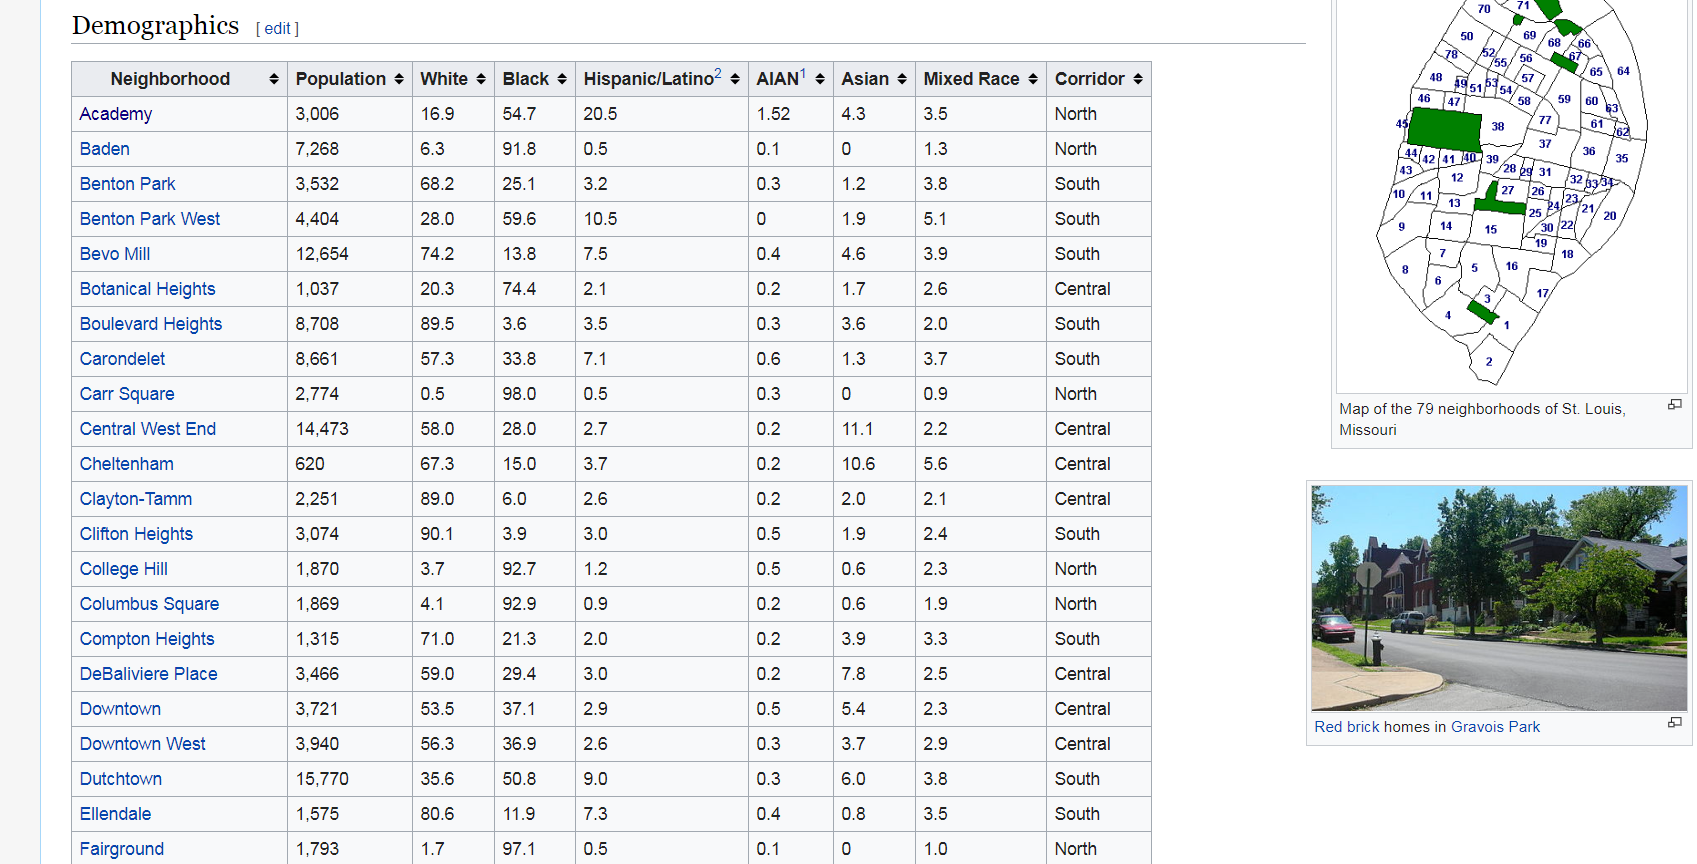
\includegraphics{Battle_of_Neighborhood_V2_files/wiki_page.png}
  \caption{A part of Wikipedia page that scoop neighborhood data}
  \label{fig:wiki_page}
\end{figure}

After downloading the data, the I created a pandas data frame. and the data frame looked like below. Notice that this is only showing the first five rows of the data for the  illustrative purposes. Numerical data are converted into int and float data types rather than having object types. Comparing the wikipedia sample above and pandas data frame below, one can identify that all the required data were downloaded properly using BeautifulSoup.


\begin{center}
\begin{figure}[h!]
  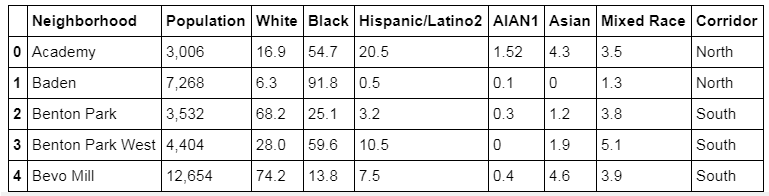
\includegraphics{Battle_of_Neighborhood_V2_files/data_read_wiki_table.png}
  % \caption{A part of Wikipedia page that scoop neighborhood data}
  % \label{fig:wiki_page}
\end{figure}
\end{center}

Notice that according to the table above, St. Louis has three regions, north, south, and central. Since the demographic data are there, it made sense to do an initial analysis of those data to find demographic concentration on each of these regions. I decided to find the average percentages of different ethnic groups living in each region mentioned above.

Following data table shows the average percentages in each corridor/region. It looks like most white people live in South side has more white people, north side is dominated by black people, Asian tends to go in the Central region. 

\begin{center}
\begin{figure}[h!]
  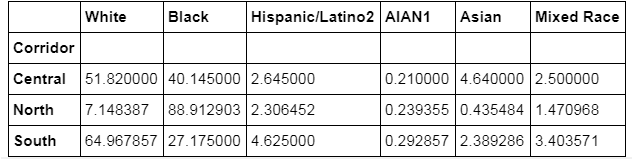
\includegraphics{Battle_of_Neighborhood_V2_files/avg_table.png}
  % \caption{A part of Wikipedia page that scoop neighborhood data}
  % \label{fig:wiki_page}
\end{figure}
\end{center}

            
This tabular data can be nicely visualize using a bar chart as shown below. With that graph it is much clear that white people dominate in north while the black people dominate in the south. The central region is almost equally distributed by both ethnicity. Other ethnic groups are not dominating in any region and create very small contributions.

    \begin{center}
    \adjustimage{max size={0.9\linewidth}{0.9\paperheight}}{Battle_of_Neighborhood_V2_files/Battle_of_Neighborhood_V2_17_0.png}
    \end{center}
    
    
    \hypertarget{obtain-the-latitude-longitude-address-and-miles-to-work-for-each-neighborhood}{%
\subsection{Obtain the latitude, longitude, address, and miles to
work for each
neighborhood}\label{obtain-the-latitude-longitude-address-and-miles-to-work-for-each-neighborhood}}

My next step was to find additional data for each neighborhood. For this section, I found Latitude, Longitude, Address, and Distance to the workplace. For this, I created a python function that will give me a pandas data frame with all the information mentioned. Following is a sample of the data frame generated using five random rows of data.

	
    \begin{center}
    \adjustimage{max size={0.9\linewidth}{0.9\paperheight}}{Battle_of_Neighborhood_V2_files/add_data.png}
    \end{center}

           
    I noticed that Nominatim doesn't always give a valid address for some
neighborhoods. This behavior can be improved by including the city and
the state with the search query. For the case of St.~Louis, I got all
the address. But in case incomplete data are there, I decided to drop
those lines with incomplete data rather than trying to search for the
address. Because the number of neighborhoods without the addresses may
not be many and additional information may not not worth the time spend
for this case.

    I also noticed that some times there were several neighborhoods was
identified by the Nomitatim is not even belongs to the state I am
searching. I am not sure the reason for these, but I think somehow
nominatim is not registering the city and the state of the search query.
One way to take care of that find those and remove them individually.
However, since I am not interested in any neighborhood more than 30
miles, I can just get rid of those, which should automatically take care
of out of the state neighborhoods.

      After both of the above processes, the number of neighborhoods still stayed 77.
That means Nominatim actually did a wonderful job of searching the
addresses of our neighborhoods. 

             
    \hypertarget{obtain-venues-around-each-neighborhood}{%
\subsection{Obtain venues around each
neighborhood}\label{obtain-venues-around-each-neighborhood}}

 	After finding the coordinates, I wanted to find good amenities around each neighborhood. I was using Fooursquare api for that. I have a free account with them which
allow me to make 100 k free requests per day. I definitely acknowledge
their service. I crated another important function accomplish this. What this function does is produce a data frame that contains the information nearby amenities, up to a 100 of those. Following data frame is the result of this function.

    
   \begin{center}
    \adjustimage{max size={0.99\linewidth}{0.9\paperheight}}{Battle_of_Neighborhood_V2_files/foursquare.png}
    \end{center}
   
            
    It looks like the function returned information about 811 venues while above table is only showing 5 venues. But it is interesting to know how many venues for each neighborhood have. I created new data frame using pandas group by function to above data frame by grouping with the Neighborhood column.  This found the total number of amenities around each neighborhood. Since I also like to know the distance from each neighborhood, I added that information to a data frame first.

\begin{center}
    \adjustimage{max size={0.5\linewidth}{0.9\paperheight}}{Battle_of_Neighborhood_V2_files/sum_venues.png}
    \end{center}

            
I plotted data to and see how the results look like. I created bar graph of
Neighborhood vs. Total number of Venues. Since I am interested about the distance to work, I displayed miles to work on top of each bar.


    \begin{center}
    \adjustimage{max size={0.99\linewidth}{0.9\paperheight}}{Battle_of_Neighborhood_V2_files/Battle_of_Neighborhood_V2_37_0.png}
    \end{center}
   
    
    According to the graph, it is clear that the top place for a lot of
amenities is Central West End which is only 3.3 miles away. Then there
is Downtown, Downtown West, etc. But the distance is not the only thing
I am looking at. I found that we had these venues belongs to 177 different unique categories.

\newpage
    \hypertarget{analyze-each-neighborhood-to-find-how-many-unique-catogories-are-belongs-to-each-neighborhood}{%
\subsection{Analyze Each Neighborhood to find how many unique
catogories are belongs to each
neighborhood}\label{analyze-each-neighborhood-to-find-how-many-unique-catogories-are-belongs-to-each-neighborhood}}

    My goal was to find the best neighborhood that has so many different
amenities close by. I was planning to use the k-means algorithm. For
that, I wanted to create another data frame that has all our
neighborhoods in the first column and frequency of different categories
of amenities in the next columns. So I should have columns equal to the
number of different categories I found from the previous section + 1
(for the Neighborhood name column). Let's creae a dummy data frame and
then we will fill the fields with the mean.
          
    It turns out that different neighborhoods have different strength as the
top comment venue for each neighborhood is different. For example, if
you are a person who likes Music you might want to go to Belleair, but
if you are someone you want to access to the gym every day, you might
find Bunker Hill is better. Did I lose you for a moment? Ok, let me show
what I mean. Let me show you what are the best 10 common venues near
each neighborhood. See below.

 \begin{center}
    \adjustimage{max size={0.99\linewidth}{0.9\paperheight}}{Battle_of_Neighborhood_V2_files/10th_best.png}
    \end{center}

   ]         
    I think by looking at the table above you might understand that
different neighborhoods have different amenities strength. The best
neighborhood depends on which kind of amenities are around you and what
your choises are.

With this, I am done with my data preperation and preliminary analysis
of the data. Let's move on to real machine learning.

\newpage
    \hypertarget{methodology---k-means-clustering}{%
\section{ Methodology - K-means
Clustering}\label{methodology---k-means-clustering}}

    For this study, I used K-means clustering algorithm. Since we
have unlabeled data, I think this will be a very good starting point to
do an unsupervised algorithm. However, I was not 100 \% sure how many
clusters to choose. I needed to do some calculations to find the best number
of clusters

    \hypertarget{choosing-the-best-cluster-number-using-elbow-method}{%
\subsection{Choosing the best cluster number using elbow
method}\label{choosing-the-best-cluster-number-using-elbow-method}}

One way to find the right number of for k is use of elbow method. I started from K = 1 and go up to K = 10 and did k-mean clustering for each K value. To find the best K value, I compared the resulted inertia or within-cluster sum-of-squares value. The following figure shows the Inertia vs k value plot.

    \begin{center}
    \adjustimage{max size={0.9\linewidth}{0.9\paperheight}}{Battle_of_Neighborhood_V2_files/Battle_of_Neighborhood_V2_54_0.png}
    \end{center}
    
    As the number of clusters increases, the centroids becomes closer to
their clusters. This makes the distortion decrease as you increase K.
You will get he minimum distortion when the number of clusters is
exactly equal to the number of data points. At that case the distortion becomes exactly
zero. But notice the graph has a sudden variation of the slope at k = 4.
Therefore, according to the Elbow method, we will consider this point as
the best number of clusters as beyond this point the improvement of
distortion is minimal.

\hypertarget{reanalize-data-with-best-k}{%
\subsection{Reanalyze data with best
K}\label{reanalize-data-with-best-k}}

Let's rerun the K-mean method with k = 3. According to the graph, one
can argue that k = 2, is more accurate. However, since the Distortion
change is significant from k = 2 to k = 3, I choose k = 3. I found that resulted clustering labels for each cluster. The labels are nicely randomly distributed. This was actually a good sign that K-means was appropriate and
working well for this problem. This can be further confirmed by plotting
all data points in the map. Just wait for it.

  
            
    \hypertarget{creating-an-interactive-map-to-show-the-neighborhoods-and-their-cluster-numbers}{%
\subsection{Creating an interactive map to show the neighborhoods
and their cluster
numbers}\label{creating-an-interactive-map-to-show-the-neigborhoods-and-their-cluster-numbers}}

Nothing beats to the interactive map of the different neighborhoods. Folium is great at producing an interactive map. Following figure showing an image of the map produced. Different color dots in the map represent the location of neighborhoods analyzed. The colors correspond to different k-mean groups. The balloon icon close to the middle of the map is showing us the location of my workplace. 

\begin{center}
    \adjustimage{max size={0.99\linewidth}{0.9\paperheight}}{Battle_of_Neighborhood_V2_files/map1.png}
    \end{center}
    
The map showing above was highly interactive. One can zoom the map to see more details around a particular neighborhood. If you click on a colored dot, it can tell you the information about that particular point. I programmed so that when you click on a point it will show us the name of the neighborhood, cluster id, and distance to work. In the figure above, I clicked on the neighborhood 'Baden'. This neighborhood belongs to category 1 and situated in 6.48 miles from my prospective workplace.
    
\newpage
            
    \hypertarget{results}{%
\section{Results}\label{results}}

The original problem was to find the best neighborhood to have less
commute time and easy access to close by venues. From a Wikipedia page,
we found that there are 79 neighborhoods around St.~Louis, Illinois. The
initial analyses of the data suggested that there are 3 main regions of
St.~Louis and different ethnic groups dominated in different areas.
North populated with black and the south is mainly occupied by white. It
is not unusual to see that the central region is roughly populated by
both groups. Other ethnic groups are scattered across all areas.

When I try to find the locations of the neighborhoods using geolocator
app, it gave me no results for two neighborhoods. I could have obtained
the locations for those two neighborhoods manually. Since it is just
less than 3 \% of the total data, I decided that not to put time on
that. On the other hand, I like to use this learning algorithm for other
towns. Therefore, it might be wise to stick to programmable solutions.

Then I obtained the amenities around each neighborhood. I found that the
total number of amenities around each neighborhood ranges from 1 to
\textasciitilde{}70. According to the plot I created, the Central West
End neighborhood has the best amenities around it with only 3.3 miles
away from the workplace. There were a total of 811 venues covering 177
unique categories.

Then I found the frequency of each venue type belongs to each
neighborhood created a new data frame. After adding the miles to work
data column to this data frame, I used to use this as the input for the
K-means algorithm.

I decided to use the K-means algorithm because of it very simple and
fast for finding similar features in unlabeled data. I search through
different values of Ks. Using the elbow method, I found that K = 3 would
give us the optimum results. All 77 neighborhoods were divided into 3
categories by K-means.

    \hypertarget{average-cluster-results}{%
\subsection{4.1 Average cluster
results}\label{average-cluster-results}}

Let's investigate these three categories (cluster labels) in more details by averaging
different numbers of data.

\begin{center}
    \adjustimage{max size={0.80\linewidth}{0.9\paperheight}}{Battle_of_Neighborhood_V2_files/avg_cluster_res.png}
    \end{center}
            
    Notice that, I did not give the demographic data as input. The reason I
didn't do it because original data suggested that different ethnic
groups are already concentrated into some parts of the town, north
-black, south -white, center -mixed. But it very interesting to notice
that both K group 0 and 3 are black-dominated, K Group 1 is black and
white roughly equally distributed. Notice that K groups are nicely
scattered around the map. If any, one can expect that all ethnics should
have mixed numbers. Yet, different K-clustering have their own identical
demographic variations, which is definitely unexpected and very
interesting. In terms of the miles to work, K group 2 have an edge. On
the other hand, the total number of venues are about the same for all
three categories. \textbf{According to these results, my personal choice
is a K - 2 group due to the closer distance to work and more close by
venues.}

\newpage
    \hypertarget{graphical-representation-of-best-neighborhoods}{%
\subsection{Graphical representation of best
Neighborhoods}\label{graphical-representation-of-best-neighborhoods}}

Let's try to visualize this graphically. I created a bar graph, similar to the one I created during the data section of documents. But this time, other than showing the miles to work on top of each bar, I like to color the bars to show the different groups, as shown in the figure bellow.



    \begin{center}
    \adjustimage{max size={0.99\linewidth}{0.9\paperheight}}{Battle_of_Neighborhood_V2_files/Battle_of_Neighborhood_V2_66_1.png}
    \end{center}
    { \hspace*{\fill} \\}
    
    Since I like group 2 and closer distance to work, I would choose
Downtown as my top spot which has 50+ closeby venues and only half a
mile away from the work. If I do not like it, then I go for Downtown
West, Forest Park South East, etc.

    \hypertarget{discussion}{%
\section{Discussion}\label{discussion}}

The K-means algorithm was successfully able to suggest the best
neighborhood to live around St.~Louis. The best neighborhoods I choose
are showing in green in the figure above. My choise of best neighborhood
based on the number of close-by venues and closer distance to the
workplace.

While demographic data were available for each neighborhood, I have not
used those data in this study. However, one might consider that it a
deciding factor and should be included in this study. There could be
multiple other things I didn't consider. Some of those things could be
access to a good public school, the ratings of the closest public
school, distance to a bus station, a train station, or an airport, crime
rates around the neighborhood, etc. If were to include those data, a
more completed model can be developed.

Also, in the east of St.~Louis there is the Illinois -Missouri border.
The neighborhoods towards east which are close to St.~Louis but not
belongs to Missuiri are not included. I think these neighborhood can be
included in the study.

    \hypertarget{conclusion}{%
\section{Conclusion}\label{conclusion}}

    Using publicly available data and K-mean machine learning algorithm, I
was able to find several prospective neighborhoods. It is incredible
that without visiting a faraway town, we can do a detailed analysis.

I choose location data of venues nearby every neighborhood in St.~Louis
to figure out the best place to live. One of the requirements I have is
to live close by to save some driving time. However, there is a huge
room to improve this algorithm by including additional data like school
ratings, crime information, distance to public transportation, etc. Not
only adding data but also eliminating redundant data is also important
by investigating each features more carefully.

All in all, I am very comfortable that this machine learning
K-clustering was very successful at providing me the best neighborhood
to live in a foreign city.

    \hypertarget{acknowladgement}{%
\section{Acknowledgment}\label{acknowladgement}}

This project was not possible without instructors from IBM - Coursera,
therefore I thank all the IBM instructors who teach the courses in Data
Science Professional Certificate. I also thank free data providers,
Wikipedia and foursquare. This application was initially developed using
IBM cloud and Watson free account and later completed in Google Colab
project. I thank both of these services.

    \hypertarget{references}{%
\section{References}\label{references}}

\begin{enumerate}
\def\labelenumi{\arabic{enumi}.}
\item
  Main data obtained from the site: \\
  `https://en.wikipedia.org/wiki/List\_of\_neighborhoods\_of\_St.\_Louis'
\item
  Scikit-learn: Machine Learning in Python, Pedregosa et al., JMLR 12,
  pp.~2825-2830, 2011
\item
  Map data provider: https://foursquare.com/
\end{enumerate}


    % Add a bibliography block to the postdoc
    
    
    
    \end{document}
